\newpage

\section*{ $^{115}$In(n,$\gamma$)$^{116}$In (Cd) }

Power Level: 100 kW(th) \\
Time at Power: 60.0 s \\
Wait Time:  4.0 h \\
Counting Time:  2.0 m \\
Total Activity at Removal: 3.02e+03 $\mu Ci$

\begin{table*}[h]
\centering
\begin{tabular}{ |c|c|c|c|c|c| }
 \hline
 Position & Mass $mg$ & Counting Activity $\mu Ci$ & Area (Counts) & Error \% \\
 \hline 
 1 & 2.20 & 2.95e+01 & 1.71e+06 & 0.0765 \\ 
\hline
 2 & 2.20 & 4.88e+01 & 2.83e+06 & 0.0594 \\ 
\hline
 3 & 2.00 & 3.84e+01 & 2.22e+06 & 0.0671 \\ 
\hline
 4 & 2.20 & 1.93e+01 & 1.12e+06 & 0.0946 \\ 
\hline
\end{tabular}
\end{table*}

\begin{figure}[h]
\centering
\begin{subfigure}{.5\textwidth}
  \centering
     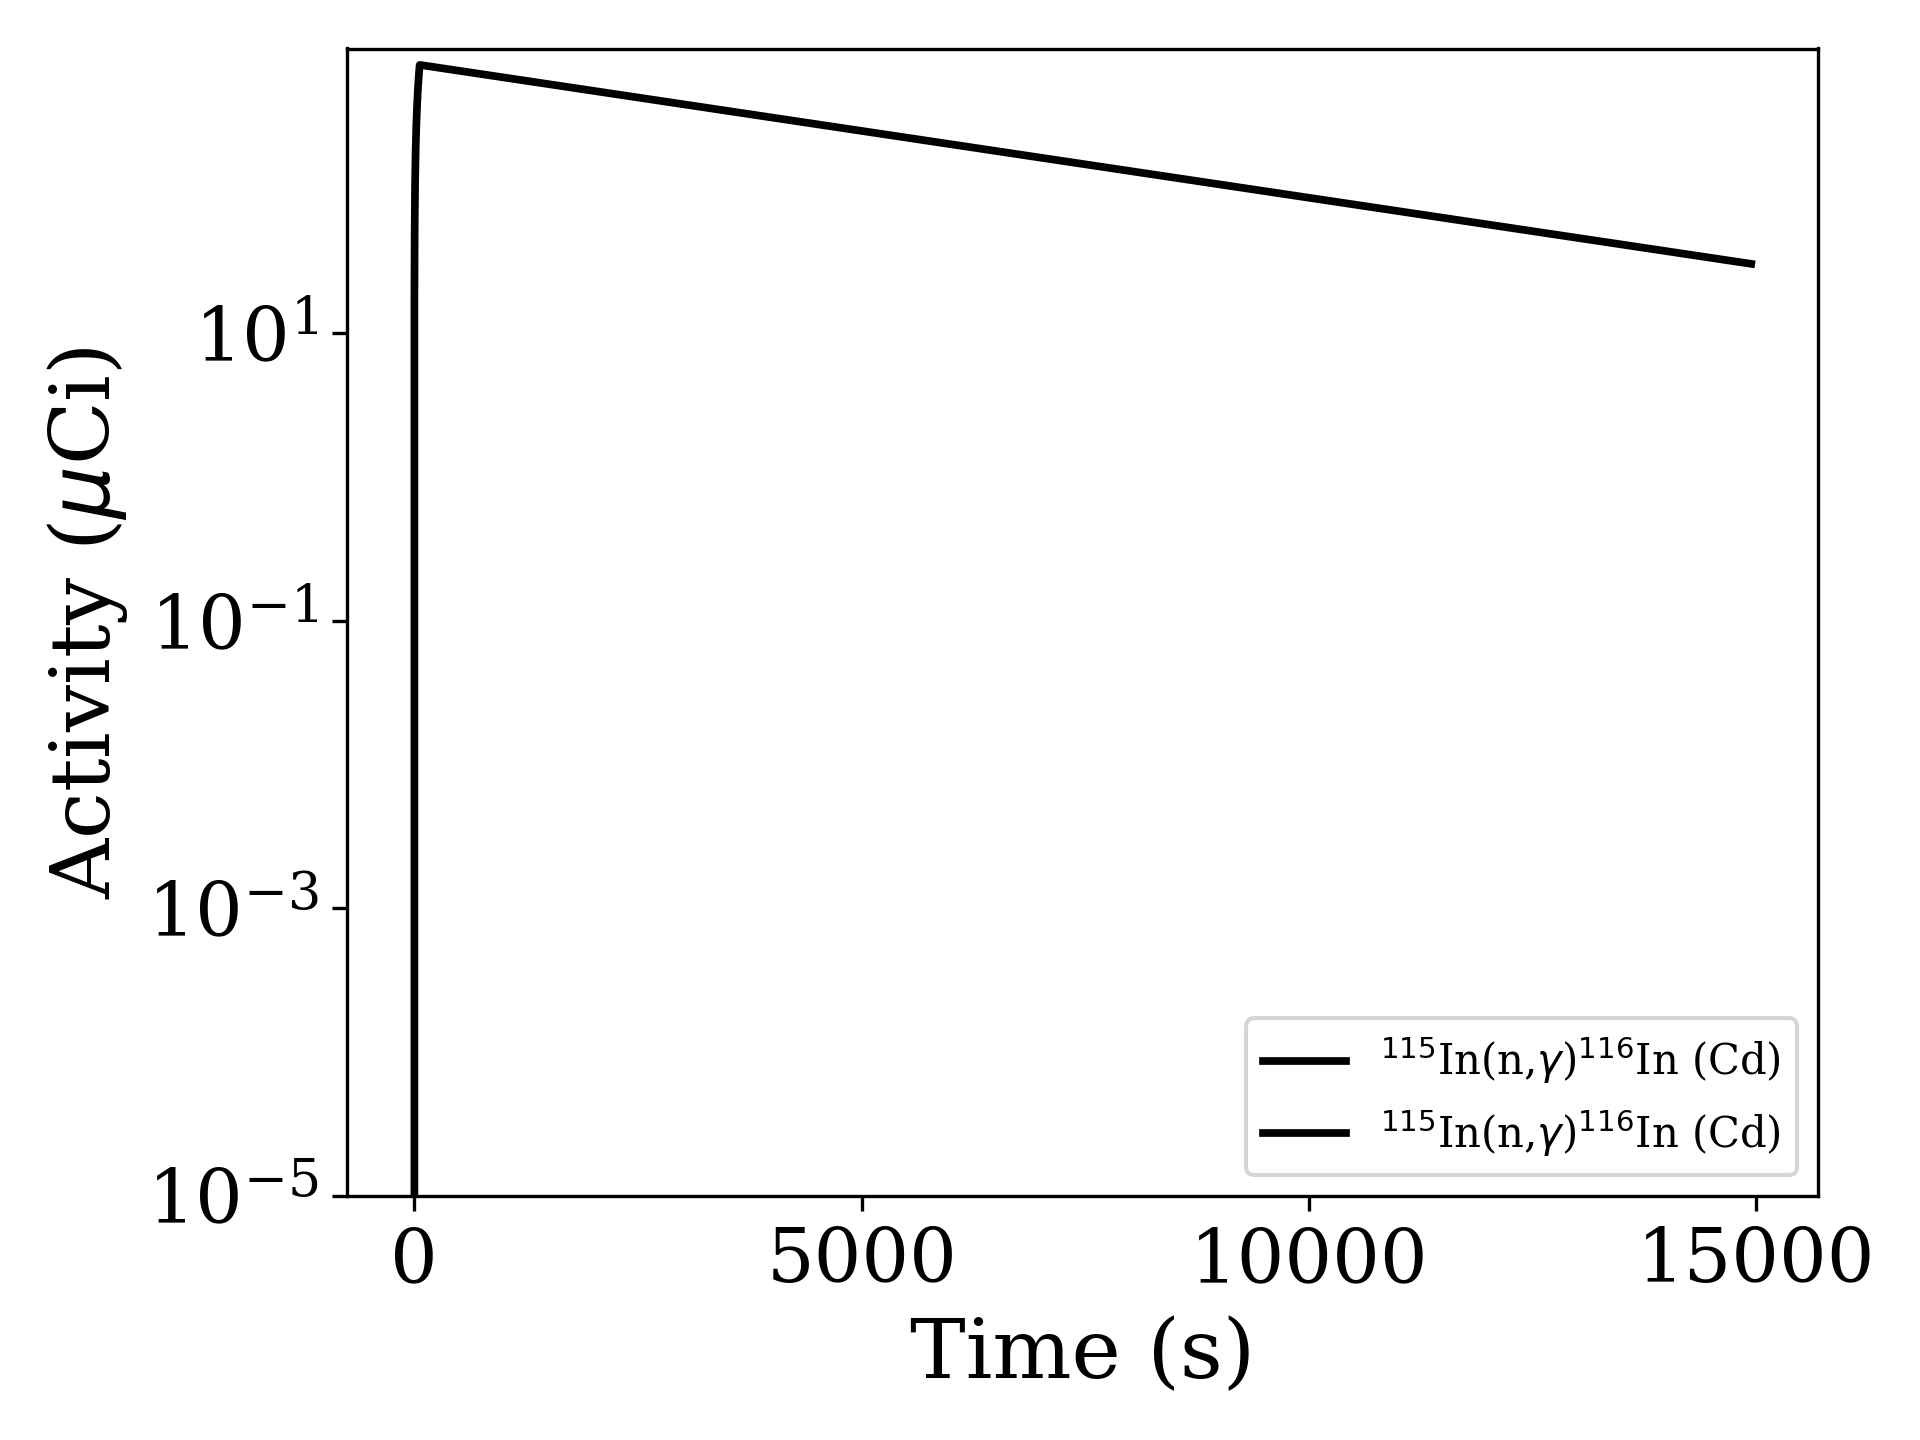
\includegraphics[width=.8\textwidth]{plot/In-115(n,gamma)In-116_Cd_wisconsin1} 

  \caption{Activity}
\end{subfigure}%
\begin{subfigure}{.5\textwidth}
  \centering
     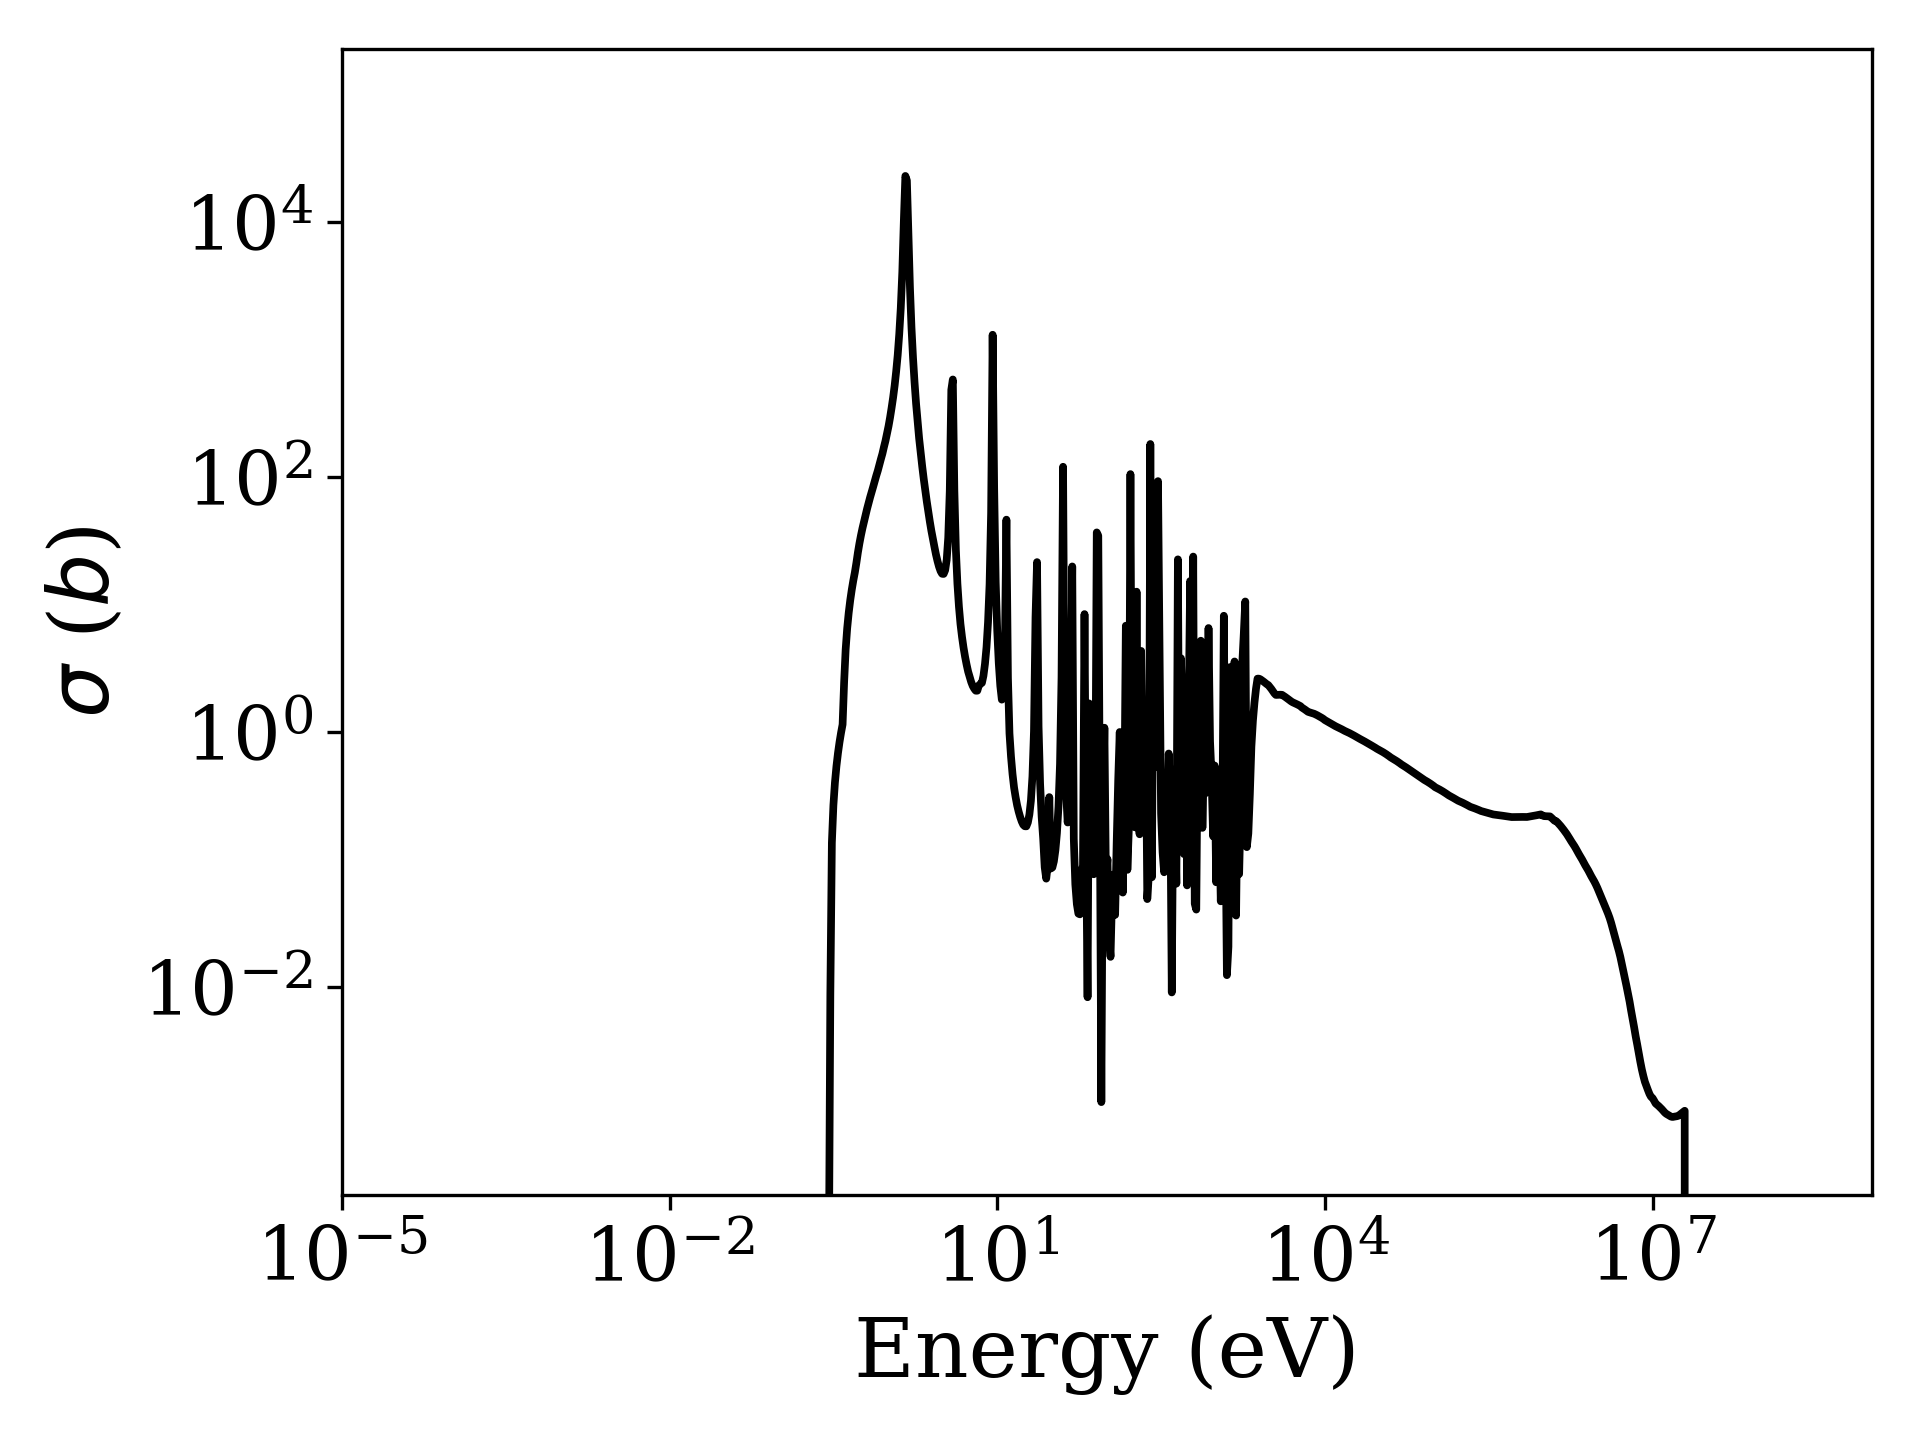
\includegraphics[width=.8\textwidth]{plot/In-115(n,gamma)In-116_Cd} 

  \caption{Cross Section}
\end{subfigure}
\end{figure}

\begin{table*}[h]
\centering
\begin{tabular}{ |c|c|c|c|c|c|c| }
 \hline
 Reaction & T$_{1/2}$ & ROI (eV) & Important Gammas (keV) \\
 \hline 
 $^{115}$In(n,$\gamma$)$^{116}$In (Cd) & 54.0 m & 1.22e+00, 1.99e+00 & 1293(0.8) \\ 
\hline
\end{tabular}
\end{table*}
